\PassOptionsToPackage{unicode=true}{hyperref} % options for packages loaded elsewhere
\PassOptionsToPackage{hyphens}{url}
%
\documentclass[10pt,ignorenonframetext,]{beamer}
\usepackage{pgfpages}
\setbeamertemplate{caption}[numbered]
\setbeamertemplate{caption label separator}{: }
\setbeamercolor{caption name}{fg=normal text.fg}
\beamertemplatenavigationsymbolsempty
% Prevent slide breaks in the middle of a paragraph:
\widowpenalties 1 10000
\raggedbottom
\setbeamertemplate{part page}{
\centering
\begin{beamercolorbox}[sep=16pt,center]{part title}
  \usebeamerfont{part title}\insertpart\par
\end{beamercolorbox}
}
\setbeamertemplate{section page}{
\centering
\begin{beamercolorbox}[sep=12pt,center]{part title}
  \usebeamerfont{section title}\insertsection\par
\end{beamercolorbox}
}
\setbeamertemplate{subsection page}{
\centering
\begin{beamercolorbox}[sep=8pt,center]{part title}
  \usebeamerfont{subsection title}\insertsubsection\par
\end{beamercolorbox}
}
\AtBeginPart{
  \frame{\partpage}
}
\AtBeginSection{
  \ifbibliography
  \else
    \frame{\sectionpage}
  \fi
}
\AtBeginSubsection{
  \frame{\subsectionpage}
}
\usepackage{lmodern}
\usepackage{amssymb,amsmath}
\usepackage{ifxetex,ifluatex}
\usepackage{fixltx2e} % provides \textsubscript
\ifnum 0\ifxetex 1\fi\ifluatex 1\fi=0 % if pdftex
  \usepackage[T1]{fontenc}
  \usepackage[utf8]{inputenc}
  \usepackage{textcomp} % provides euro and other symbols
\else % if luatex or xelatex
  \usepackage{unicode-math}
  \defaultfontfeatures{Ligatures=TeX,Scale=MatchLowercase}
\fi
\usetheme[]{Madrid}
% use upquote if available, for straight quotes in verbatim environments
\IfFileExists{upquote.sty}{\usepackage{upquote}}{}
% use microtype if available
\IfFileExists{microtype.sty}{%
\usepackage[]{microtype}
\UseMicrotypeSet[protrusion]{basicmath} % disable protrusion for tt fonts
}{}
\IfFileExists{parskip.sty}{%
\usepackage{parskip}
}{% else
\setlength{\parindent}{0pt}
\setlength{\parskip}{6pt plus 2pt minus 1pt}
}
\usepackage{hyperref}
\hypersetup{
            pdftitle={Tidying Data in R},
            pdfauthor={Bas Machielsen},
            pdfborder={0 0 0},
            breaklinks=true}
\urlstyle{same}  % don't use monospace font for urls
\newif\ifbibliography
\usepackage{color}
\usepackage{fancyvrb}
\newcommand{\VerbBar}{|}
\newcommand{\VERB}{\Verb[commandchars=\\\{\}]}
\DefineVerbatimEnvironment{Highlighting}{Verbatim}{commandchars=\\\{\}}
% Add ',fontsize=\small' for more characters per line
\usepackage{framed}
\definecolor{shadecolor}{RGB}{248,248,248}
\newenvironment{Shaded}{\begin{snugshade}}{\end{snugshade}}
\newcommand{\AlertTok}[1]{\textcolor[rgb]{0.94,0.16,0.16}{#1}}
\newcommand{\AnnotationTok}[1]{\textcolor[rgb]{0.56,0.35,0.01}{\textbf{\textit{#1}}}}
\newcommand{\AttributeTok}[1]{\textcolor[rgb]{0.77,0.63,0.00}{#1}}
\newcommand{\BaseNTok}[1]{\textcolor[rgb]{0.00,0.00,0.81}{#1}}
\newcommand{\BuiltInTok}[1]{#1}
\newcommand{\CharTok}[1]{\textcolor[rgb]{0.31,0.60,0.02}{#1}}
\newcommand{\CommentTok}[1]{\textcolor[rgb]{0.56,0.35,0.01}{\textit{#1}}}
\newcommand{\CommentVarTok}[1]{\textcolor[rgb]{0.56,0.35,0.01}{\textbf{\textit{#1}}}}
\newcommand{\ConstantTok}[1]{\textcolor[rgb]{0.00,0.00,0.00}{#1}}
\newcommand{\ControlFlowTok}[1]{\textcolor[rgb]{0.13,0.29,0.53}{\textbf{#1}}}
\newcommand{\DataTypeTok}[1]{\textcolor[rgb]{0.13,0.29,0.53}{#1}}
\newcommand{\DecValTok}[1]{\textcolor[rgb]{0.00,0.00,0.81}{#1}}
\newcommand{\DocumentationTok}[1]{\textcolor[rgb]{0.56,0.35,0.01}{\textbf{\textit{#1}}}}
\newcommand{\ErrorTok}[1]{\textcolor[rgb]{0.64,0.00,0.00}{\textbf{#1}}}
\newcommand{\ExtensionTok}[1]{#1}
\newcommand{\FloatTok}[1]{\textcolor[rgb]{0.00,0.00,0.81}{#1}}
\newcommand{\FunctionTok}[1]{\textcolor[rgb]{0.00,0.00,0.00}{#1}}
\newcommand{\ImportTok}[1]{#1}
\newcommand{\InformationTok}[1]{\textcolor[rgb]{0.56,0.35,0.01}{\textbf{\textit{#1}}}}
\newcommand{\KeywordTok}[1]{\textcolor[rgb]{0.13,0.29,0.53}{\textbf{#1}}}
\newcommand{\NormalTok}[1]{#1}
\newcommand{\OperatorTok}[1]{\textcolor[rgb]{0.81,0.36,0.00}{\textbf{#1}}}
\newcommand{\OtherTok}[1]{\textcolor[rgb]{0.56,0.35,0.01}{#1}}
\newcommand{\PreprocessorTok}[1]{\textcolor[rgb]{0.56,0.35,0.01}{\textit{#1}}}
\newcommand{\RegionMarkerTok}[1]{#1}
\newcommand{\SpecialCharTok}[1]{\textcolor[rgb]{0.00,0.00,0.00}{#1}}
\newcommand{\SpecialStringTok}[1]{\textcolor[rgb]{0.31,0.60,0.02}{#1}}
\newcommand{\StringTok}[1]{\textcolor[rgb]{0.31,0.60,0.02}{#1}}
\newcommand{\VariableTok}[1]{\textcolor[rgb]{0.00,0.00,0.00}{#1}}
\newcommand{\VerbatimStringTok}[1]{\textcolor[rgb]{0.31,0.60,0.02}{#1}}
\newcommand{\WarningTok}[1]{\textcolor[rgb]{0.56,0.35,0.01}{\textbf{\textit{#1}}}}
\usepackage{graphicx,grffile}
\makeatletter
\def\maxwidth{\ifdim\Gin@nat@width>\linewidth\linewidth\else\Gin@nat@width\fi}
\def\maxheight{\ifdim\Gin@nat@height>\textheight\textheight\else\Gin@nat@height\fi}
\makeatother
% Scale images if necessary, so that they will not overflow the page
% margins by default, and it is still possible to overwrite the defaults
% using explicit options in \includegraphics[width, height, ...]{}
\setkeys{Gin}{width=\maxwidth,height=\maxheight,keepaspectratio}
\setlength{\emergencystretch}{3em}  % prevent overfull lines
\providecommand{\tightlist}{%
  \setlength{\itemsep}{0pt}\setlength{\parskip}{0pt}}
\setcounter{secnumdepth}{0}

% set default figure placement to htbp
\makeatletter
\def\fps@figure{htbp}
\makeatother

\usepackage{booktabs}
\usepackage{longtable}
\usepackage{array}
\usepackage{multirow}
\usepackage{wrapfig}
\usepackage{float}
\usepackage{colortbl}
\usepackage{pdflscape}
\usepackage{tabu}
\usepackage{threeparttable}
\usepackage{threeparttablex}
\usepackage[normalem]{ulem}
\usepackage{makecell}
\usepackage{xcolor}

\title{Tidying Data in R}
\author{Bas Machielsen}
\providecommand{\institute}[1]{}
\institute{Utrecht University}
\date{\today}

\begin{document}
\frame{\titlepage}

\begin{frame}[fragile]{What is tidy data?}
\protect\hypertarget{what-is-tidy-data}{}

\begin{itemize}
\item
  In order for your data to be ready for analysis, it needs to be
  \textbf{tidy}.
\item
  Tidy data is defined as:
\end{itemize}

\begin{quote}
data sets that are arranged such that each variable is a column and each
observation (or case) is a row.
\end{quote}

\begin{itemize}
\item
  I will attempt to explain how to put this principle in practice using
  a set of packages called the \textbf{tidyverse}, but strictly
  speaking, only the \texttt{tidyr} package is required.
\item
  You can download the .Rmd and .csv files from my
  \href{www.github.com/basm92}{\textbf{github page}}, and follow along!
\end{itemize}

\end{frame}

\begin{frame}{What is (un)tidy data?}
\protect\hypertarget{what-is-untidy-data}{}

\begin{quote}
All tidy data are similar to each other. All untidy data are untidy in
their own way.
\end{quote}

\begin{itemize}
\item
  Although tidy data shares the properties mentioned in the previous
  slide, untidy data refers (broadly speaking) to unstructured data.
\item
  An example (from \url{www.tidyverse.org}):
\end{itemize}

\begin{table}

\caption{\label{tab:unnamed-chunk-1}This is what an untidy dataset looks like}
\centering
\begin{tabular}[t]{lrr}
\toprule
name & treatmenta & treatmentb\\
\midrule
\rowcolor{gray!6}  John Smith & NA & 18\\
Jane Doe & 4 & 1\\
\rowcolor{gray!6}  Mary Johnson & 6 & 7\\
\bottomrule
\end{tabular}
\end{table}

\end{frame}

\begin{frame}{An example of untidy data}
\protect\hypertarget{an-example-of-untidy-data}{}

\begin{itemize}
\item
  Is each obervation in a row?
\item
  Is each variable in a column?
\item
  What are the variables here?
\end{itemize}

\begin{table}

\caption{\label{tab:unnamed-chunk-2}This is also what an untidy dataset looks like}
\centering
\begin{tabular}[t]{lrrr}
\toprule
treatment & John.Smith & Jane.Doe & Mary.Johnson\\
\midrule
\rowcolor{gray!6}  a & NA & 4 & 6\\
b & 18 & 1 & 7\\
\bottomrule
\end{tabular}
\end{table}

\end{frame}

\begin{frame}[fragile]{Example: from untidy to tidy data}
\protect\hypertarget{example-from-untidy-to-tidy-data}{}

\begin{itemize}
\tightlist
\item
  The variables are (i) the treatment, (ii) the subject, and (iii) the
  `score' corresponding to each subject-treatment observations.
\end{itemize}

\begin{Shaded}
\begin{Highlighting}[]
\NormalTok{preg }\OperatorTok
\StringTok{    }\KeywordTok{pivot_longer}\NormalTok{(treatmenta}\OperatorTok{:}\NormalTok{treatmentb, }
                 \DataTypeTok{names_to =} \StringTok{"treatment"}\NormalTok{, }\DataTypeTok{values_to =} \StringTok{"score"}\NormalTok{) }\OperatorTok\StringTok{ }
\StringTok{    }\KeywordTok{mutate}\NormalTok{(}\DataTypeTok{treatment =} \KeywordTok{gsub}\NormalTok{(}\StringTok{"treatment"}\NormalTok{, }\StringTok{""}\NormalTok{, treatment)) }\OperatorTok
\StringTok{    }\KeywordTok{arrange}\NormalTok{(name, treatment) }\OperatorTok
\StringTok{    }\KeywordTok{kable}\NormalTok{(}\DataTypeTok{caption =} \StringTok{"Test"}\NormalTok{, }\DataTypeTok{booktabs =} \OtherTok{TRUE}\NormalTok{, }
          \DataTypeTok{row.names =} \OtherTok{FALSE}\NormalTok{) }\OperatorTok
\StringTok{    }\KeywordTok{kable_styling}\NormalTok{(}\DataTypeTok{latex_options =} \StringTok{"striped"}\NormalTok{)}
\end{Highlighting}
\end{Shaded}

\end{frame}

\begin{frame}{Example: from untidy to tidy data}
\protect\hypertarget{example-from-untidy-to-tidy-data-1}{}

\begin{itemize}
\tightlist
\item
  The former chunk of code transforms the data in the first table to the
  following table:
\end{itemize}

\begin{table}

\caption{\label{tab:unnamed-chunk-4}This is tidy data}
\centering
\begin{tabular}[t]{llr}
\toprule
name & treatment & score\\
\midrule
\rowcolor{gray!6}  Jane Doe & a & 4\\
Jane Doe & b & 1\\
\rowcolor{gray!6}  John Smith & a & NA\\
John Smith & b & 18\\
\rowcolor{gray!6}  Mary Johnson & a & 6\\
\addlinespace
Mary Johnson & b & 7\\
\bottomrule
\end{tabular}
\end{table}

\end{frame}

\begin{frame}[fragile]{Transforming the data}
\protect\hypertarget{transforming-the-data}{}

\begin{itemize}
\item
  The key command in the former chunk of code is \texttt{pivot\_longer}.
  With the arguements data, columns, names\_to and values\_to.
\item
  All the other functions are essentially layout changes, not
  fundamental transformations.
\item
  The command pivot\_longer basically transforms the dataset from:
\end{itemize}

\begin{table}

\caption{\label{tab:unnamed-chunk-5}This is what an untidy dataset looks like}
\centering
\begin{tabular}[t]{lrr}
\toprule
name & treatmenta & treatmentb\\
\midrule
\rowcolor{gray!6}  John Smith & NA & 18\\
Jane Doe & 4 & 1\\
\rowcolor{gray!6}  Mary Johnson & 6 & 7\\
\bottomrule
\end{tabular}
\end{table}

\end{frame}

\begin{frame}[fragile]{Transforming the data}
\protect\hypertarget{transforming-the-data-1}{}

\begin{itemize}
\tightlist
\item
  to :
\end{itemize}

\begin{Shaded}
\begin{Highlighting}[]
\KeywordTok{pivot_longer}\NormalTok{(}\DataTypeTok{data =}\NormalTok{ preg, }\DataTypeTok{cols =} \DecValTok{2}\OperatorTok{:}\DecValTok{3}\NormalTok{, }\DataTypeTok{names_to =} \StringTok{"treatment"}\NormalTok{, }
             \DataTypeTok{values_to =} \StringTok{"score"}\NormalTok{) }\OperatorTok
\StringTok{    }\KeywordTok{kable}\NormalTok{(}\DataTypeTok{caption =} \StringTok{"This is what a tidy dataset looks like"}\NormalTok{, }
      \DataTypeTok{booktabs =} \OtherTok{TRUE}\NormalTok{, }\DataTypeTok{row.names =} \OtherTok{FALSE}\NormalTok{) }\OperatorTok
\StringTok{  }\KeywordTok{kable_styling}\NormalTok{(}\DataTypeTok{latex_options =} \StringTok{"striped"}\NormalTok{)}
\end{Highlighting}
\end{Shaded}

\begin{table}

\caption{\label{tab:unnamed-chunk-6}This is what a tidy dataset looks like}
\centering
\begin{tabular}[t]{llr}
\toprule
name & treatment & score\\
\midrule
\rowcolor{gray!6}  John Smith & treatmenta & NA\\
John Smith & treatmentb & 18\\
\rowcolor{gray!6}  Jane Doe & treatmenta & 4\\
Jane Doe & treatmentb & 1\\
\rowcolor{gray!6}  Mary Johnson & treatmenta & 6\\
\addlinespace
Mary Johnson & treatmentb & 7\\
\bottomrule
\end{tabular}
\end{table}

\end{frame}

\begin{frame}{Contents}
\protect\hypertarget{contents}{}

\begin{itemize}
\item
  The best way to see how tidy data works is by using examples. In this
  lecture, I will demonstrate extensively how to create tidy data that
  is ready for analysis using two examples.
\item
  First, I will show how to combine and tidy data on economic
  development from the World Bank.
\item
  Afterwards, I show how to combine and tidy data from Amadeus, a
  commercial database.
\item
  On the fly, I will demonstrate how simple it is to analyze or create
  graphs with tidy data.
\item
  Finally, I will use other examples to show how to tidy more messy
  data, inspired by examples from the
  \href{https://tidyr.tidyverse.org/reference/pivot_longer.html}{\textbf{tidyverse
  website}}
\end{itemize}

\end{frame}

\begin{frame}[fragile]{World Bank Dataset}
\protect\hypertarget{world-bank-dataset}{}

\begin{itemize}
\item
  Let us now download some data from the World Bank database. I extract
  the 55 basic World Development Indicators from
  \href{https://databank.worldbank.org/source/world-development-indicators/}{\textbf{here}}
  for 20 countries.
\item
  Importing the data..
\end{itemize}

\begin{Shaded}
\begin{Highlighting}[]
\NormalTok{worldbank <-}\StringTok{ }\KeywordTok{read_csv}\NormalTok{(}\StringTok{"wb.csv"}\NormalTok{)}

\KeywordTok{dim}\NormalTok{(worldbank)}
\end{Highlighting}
\end{Shaded}

\begin{verbatim}
## [1] 1105   14
\end{verbatim}

\begin{itemize}
\tightlist
\item
  The data has 1105 observations and 14 variables. That is not at all
  what we wanted. What do the data look like?
\end{itemize}

\end{frame}

\begin{frame}[fragile]{World Bank Dataset}
\protect\hypertarget{world-bank-dataset-1}{}

\begin{Shaded}
\begin{Highlighting}[]
\KeywordTok{kable}\NormalTok{(worldbank[}\DecValTok{1}\OperatorTok{:}\DecValTok{4}\NormalTok{,}\KeywordTok{c}\NormalTok{(}\DecValTok{1}\NormalTok{,}\DecValTok{2}\NormalTok{,}\DecValTok{4}\NormalTok{,}\DecValTok{5}\NormalTok{)], }
      \DataTypeTok{caption =} \StringTok{"Work Bank Data - Untidy!"}\NormalTok{, }
      \DataTypeTok{booktabs =} \OtherTok{TRUE}\NormalTok{, }\DataTypeTok{row.names =} \OtherTok{FALSE}\NormalTok{) }\OperatorTok
\StringTok{  }\KeywordTok{kable_styling}\NormalTok{(}\DataTypeTok{latex_options =} \StringTok{"striped"}\NormalTok{)}
\end{Highlighting}
\end{Shaded}

\begin{table}

\caption{\label{tab:unnamed-chunk-8}Work Bank Data - Untidy!}
\centering
\begin{tabular}[t]{llll}
\toprule
Country Name & Country Code & Series Code & 2009 [YR2009]\\
\midrule
\rowcolor{gray!6}  Argentina & ARG & SP.ADO.TFRT & 63.1896\\
Argentina & ARG & NV.AGR.TOTL.ZS & 5.27362346890139\\
\rowcolor{gray!6}  Argentina & ARG & ER.H2O.FWTL.ZS & ..\\
Argentina & ARG & SH.STA.BRTC.ZS & 97.9\\
\bottomrule
\end{tabular}
\end{table}

\begin{itemize}
\item
  Very untidy dataset! NA observations are entered as \texttt{..}, and
  variable names require an extensive definition before you know what
  they mean.
\item
  Furthermore, years are not notated straightforwardly, and the data
  violates the tidy data principles.
\end{itemize}

\end{frame}

\begin{frame}[fragile]{What to do?}
\protect\hypertarget{what-to-do}{}

\begin{itemize}
\tightlist
\item
  First, let us try to save the variable names and series code to
  another dataset (step 1), and delete the names from the worldbank
  dataset (step 2).
\end{itemize}

\begin{Shaded}
\begin{Highlighting}[]
\CommentTok{#Step 1}
\NormalTok{wbnames <-}\StringTok{ }\KeywordTok{cbind}\NormalTok{(}\KeywordTok{unique}\NormalTok{(worldbank[,}\DecValTok{3}\NormalTok{]),}\KeywordTok{unique}\NormalTok{(worldbank[,}\DecValTok{4}\NormalTok{])) }\OperatorTok
\StringTok{    }\KeywordTok{na.omit}\NormalTok{()}

\CommentTok{#Step 2}
\NormalTok{worldbank <-}\StringTok{ }\NormalTok{worldbank[}\DecValTok{1}\OperatorTok{:}\DecValTok{1100}\NormalTok{,}\OperatorTok{-}\DecValTok{3}\NormalTok{]}
\end{Highlighting}
\end{Shaded}

\end{frame}

\begin{frame}[fragile]{Almost there..}
\protect\hypertarget{almost-there..}{}

\begin{itemize}
\tightlist
\item
  Now, let's try to unpivot the columns containing the years..
\end{itemize}

\begin{Shaded}
\begin{Highlighting}[]
\NormalTok{worldbank <-}\StringTok{ }\KeywordTok{pivot_longer}\NormalTok{(worldbank, }\DecValTok{4}\OperatorTok{:}\DecValTok{13}\NormalTok{, }
             \DataTypeTok{names_to =} \StringTok{"years"}\NormalTok{, }
             \DataTypeTok{values_to =} \StringTok{"value"}\NormalTok{)}
\end{Highlighting}
\end{Shaded}

\begin{itemize}
\tightlist
\item
  This is what the data looks like right now.
\end{itemize}

\begin{table}

\caption{\label{tab:unnamed-chunk-11}The data then looks like this.}
\centering
\begin{tabular}[t]{llll}
\toprule
Country Code & Series Code & years & value\\
\midrule
\rowcolor{gray!6}  ARG & SP.ADO.TFRT & 2009 [YR2009] & 63.1896\\
ARG & SP.ADO.TFRT & 2010 [YR2010] & 63.3154\\
\rowcolor{gray!6}  ARG & SP.ADO.TFRT & 2011 [YR2011] & 63.4412\\
ARG & SP.ADO.TFRT & 2012 [YR2012] & 63.567\\
\bottomrule
\end{tabular}
\end{table}

\end{frame}

\begin{frame}[fragile]{Final steps}
\protect\hypertarget{final-steps}{}

\begin{itemize}
\item
  Let's now clean the ``years'' variable (step 1), set the \texttt{..}
  observations to NA (step 2), and ``widen'' the data so that every
  separate indicator gets a column (step 3).
\item
  Step 3 is done using the \texttt{pivot\_wider} command: it widens the
  data and shortens the number of observations, because it transfers
  information from rows to columns.
\end{itemize}

\begin{Shaded}
\begin{Highlighting}[]
\CommentTok{#Step 1}
\NormalTok{worldbank <-}\StringTok{ }\NormalTok{worldbank }\OperatorTok
\StringTok{    }\KeywordTok{mutate}\NormalTok{(}\DataTypeTok{years =} \KeywordTok{substring}\NormalTok{(years, }\DecValTok{1}\NormalTok{, }\DecValTok{4}\NormalTok{))}

\CommentTok{#Step 2}
\NormalTok{worldbank}\OperatorTok{$}\NormalTok{value[worldbank}\OperatorTok{$}\NormalTok{value }\OperatorTok{==}\StringTok{ ".."}\NormalTok{] <-}\StringTok{ }\OtherTok{NA}

\CommentTok{#Step 3}
\NormalTok{worldbank <-}\StringTok{ }\KeywordTok{pivot_wider}\NormalTok{(}\DataTypeTok{data =}\NormalTok{ worldbank,}
                         \DataTypeTok{names_from =} \StringTok{`}\DataTypeTok{Series Code}\StringTok{`}\NormalTok{,}
                         \DataTypeTok{values_from =} \StringTok{`}\DataTypeTok{value}\StringTok{`}\NormalTok{)}
\end{Highlighting}
\end{Shaded}

\end{frame}

\begin{frame}[fragile]{Done!}
\protect\hypertarget{done}{}

\begin{itemize}
\item
  \texttt{pivot\_wider}, takes three arguments: the data, from which
  column it should take the new column names (names\_from), and from
  which column it should take the values belonging to the corresonding
  cels (values\_from).
\item
  This is what it looks like!
\end{itemize}

\begin{table}

\caption{\label{tab:unnamed-chunk-13}Tidy Data}
\centering
\begin{tabular}[t]{lllll}
\toprule
Country Name & Country Code & years & SP.ADO.TFRT & NV.AGR.TOTL.ZS\\
\midrule
\rowcolor{gray!6}  Argentina & ARG & 2009 & 63.1896 & 5.27362346890139\\
Argentina & ARG & 2010 & 63.3154 & 7.13216745078964\\
\rowcolor{gray!6}  Argentina & ARG & 2011 & 63.4412 & 6.99873377022519\\
Argentina & ARG & 2012 & 63.567 & 5.7817442068501\\
\bottomrule
\end{tabular}
\end{table}

\end{frame}

\begin{frame}[fragile]{Military Spending}
\protect\hypertarget{military-spending}{}

\begin{itemize}
\item
  Suppose I want to know the military expenditures as a percentage of
  GDP MS.MIL.XPND.GD.ZS for each country in the dataset in 2015.
\item
  I can use the \texttt{wbnames} information we've saved to add labels
  to the data.
\end{itemize}

\begin{Shaded}
\begin{Highlighting}[]
\NormalTok{worldbank }\OperatorTok
\StringTok{    }\KeywordTok{filter}\NormalTok{(years }\OperatorTok{==}\StringTok{ "2015"}\NormalTok{) }\OperatorTok
\StringTok{    }\KeywordTok{ggplot}\NormalTok{(}\KeywordTok{aes}\NormalTok{(}\DataTypeTok{x =} \StringTok{`}\DataTypeTok{Country Code}\StringTok{`}\NormalTok{, }\DataTypeTok{y =} \StringTok{`}\DataTypeTok{MS.MIL.XPND.GD.ZS}\StringTok{`}\NormalTok{)) }\OperatorTok{+}\StringTok{ }
\StringTok{    }\KeywordTok{geom_col}\NormalTok{() }\OperatorTok{+}\StringTok{ }
\StringTok{    }\KeywordTok{labs}\NormalTok{(}\DataTypeTok{y =} \KeywordTok{as.character}\NormalTok{(wbnames[}\KeywordTok{match}\NormalTok{(}\StringTok{"MS.MIL.XPND.GD.ZS"}\NormalTok{,}
\NormalTok{                                        wbnames[,}\DecValTok{2}\NormalTok{]),}\DecValTok{1}\NormalTok{])) }\OperatorTok{+}
\StringTok{    }\KeywordTok{theme}\NormalTok{(}\DataTypeTok{axis.text.y =}\KeywordTok{element_blank}\NormalTok{())}
\end{Highlighting}
\end{Shaded}

\end{frame}

\begin{frame}{Military Spending}
\protect\hypertarget{military-spending-1}{}

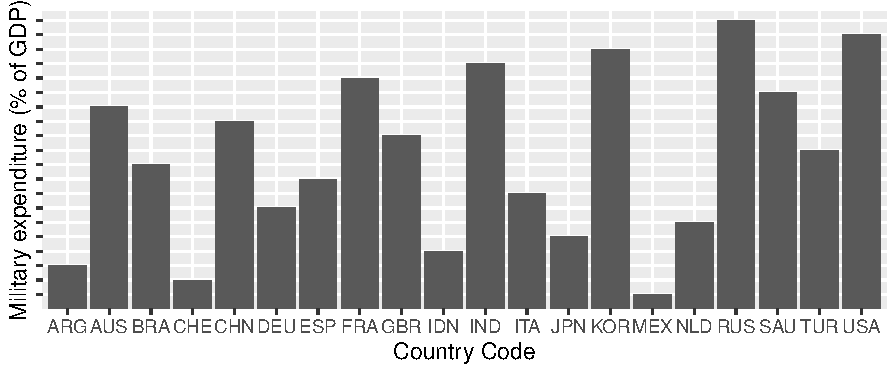
\includegraphics{PresentationTidyData_files/figure-beamer/unnamed-chunk-15-1.pdf}

\end{frame}

\begin{frame}[fragile]{Fertility Rate}
\protect\hypertarget{fertility-rate}{}

\begin{itemize}
\tightlist
\item
  Suppose now you want to track the evolution of the fertility rate over
  the last 10 years of some countries in the dataset.
\end{itemize}

\begin{Shaded}
\begin{Highlighting}[]
\NormalTok{worldbank }\OperatorTok
\StringTok{    }\KeywordTok{filter}\NormalTok{(years }\OperatorTok{<}\StringTok{ }\DecValTok{2018}\NormalTok{, }
           \StringTok{`}\DataTypeTok{Country Code}\StringTok{`} \OperatorTok{==}\StringTok{ "CHE"} \OperatorTok{|}\StringTok{ }
\StringTok{             `}\DataTypeTok{Country Code}\StringTok{`} \OperatorTok{==}\StringTok{ "GBR"}
           \OperatorTok{|}\StringTok{ `}\DataTypeTok{Country Code}\StringTok{`} \OperatorTok{==}\StringTok{ "RUS"} \OperatorTok{|}\StringTok{ }
\StringTok{             `}\DataTypeTok{Country Code}\StringTok{`} \OperatorTok{==}\StringTok{ "SAU"}\NormalTok{) }\OperatorTok
\StringTok{    }\KeywordTok{ggplot}\NormalTok{(}\KeywordTok{aes}\NormalTok{(}\DataTypeTok{x =}\NormalTok{ years, }\DataTypeTok{y =} \StringTok{`}\DataTypeTok{SP.DYN.TFRT.IN}\StringTok{`}\NormalTok{, }
               \DataTypeTok{group =} \StringTok{`}\DataTypeTok{Country Code}\StringTok{`}\NormalTok{, }
               \DataTypeTok{color =} \StringTok{`}\DataTypeTok{Country Code}\StringTok{`}\NormalTok{)) }\OperatorTok{+}\StringTok{ }
\StringTok{    }\KeywordTok{geom_line}\NormalTok{() }\OperatorTok{+}\StringTok{ }
\StringTok{    }\KeywordTok{labs}\NormalTok{(}\DataTypeTok{y =} \KeywordTok{as.character}\NormalTok{(wbnames[}\KeywordTok{match}\NormalTok{(}\StringTok{"SP.DYN.TFRT.IN"}\NormalTok{,}
\NormalTok{                                        wbnames[,}\DecValTok{2}\NormalTok{]),}\DecValTok{1}\NormalTok{])) }\OperatorTok{+}
\StringTok{    }\KeywordTok{theme}\NormalTok{(}\DataTypeTok{axis.text.y =}\KeywordTok{element_blank}\NormalTok{(), }
          \DataTypeTok{axis.ticks.y =} \KeywordTok{element_blank}\NormalTok{())}
\end{Highlighting}
\end{Shaded}

\end{frame}

\begin{frame}{Fertility Rate}
\protect\hypertarget{fertility-rate-1}{}

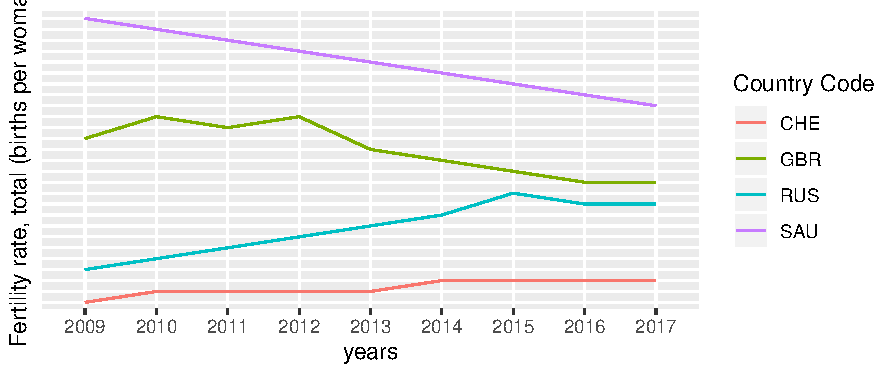
\includegraphics{PresentationTidyData_files/figure-beamer/unnamed-chunk-17-1.pdf}

\end{frame}

\begin{frame}[fragile]{Another untidy dataset..}
\protect\hypertarget{another-untidy-dataset..}{}

\begin{itemize}
\item
  Now, I will download some data from Amadeus, a commercial database
  collected information about firms across the world.
\item
  I collect data from 2000 European companies on their financial
  information, the number of employees, and the number of
  directors/managers.
\end{itemize}

\begin{Shaded}
\begin{Highlighting}[]
\NormalTok{amadeus <-}\StringTok{ }\KeywordTok{read.csv}\NormalTok{(}\StringTok{"Amadeus_Export_1.csv"}\NormalTok{, }\DataTypeTok{fileEncoding =} \StringTok{"UCS-2LE"}\NormalTok{)}

\KeywordTok{dim}\NormalTok{(amadeus)}
\end{Highlighting}
\end{Shaded}

\begin{verbatim}
## [1] 2000   68
\end{verbatim}

\end{frame}

\begin{frame}{What does the data look like?}
\protect\hypertarget{what-does-the-data-look-like}{}

\begin{itemize}
\tightlist
\item
  These are some of the variables..
\end{itemize}

\begin{table}

\caption{\label{tab:unnamed-chunk-19}Variable names}
\centering
\begin{tabular}[t]{l}
\toprule
\\
\midrule
\rowcolor{gray!6}  Mark\\
Company.name\\
\rowcolor{gray!6}  City\\
Country.ISO.code\\
\rowcolor{gray!6}  NACE.code\\
\addlinespace
Cons..code\\
\rowcolor{gray!6}  Last.year\\
Operating.revenue..Turnover..th.EUR.2019\\
\rowcolor{gray!6}  Operating.revenue..Turnover..th.EUR.2018\\
\bottomrule
\end{tabular}
\end{table}

\end{frame}

\begin{frame}[fragile]{Tidying the Amadeus data}
\protect\hypertarget{tidying-the-amadeus-data}{}

\begin{itemize}
\item
  The data look very untidy. Column names contain variables and years,
  and there are various superfluous columns, such as \texttt{Mark}, and
  last year. NA observations are coded as \texttt{n.a.} but are not
  recognized by are as such.
\item
  The first thing we need to do is to change the NA obs to functioning
  NA obs, and remove some superfluous columns
\end{itemize}

\begin{Shaded}
\begin{Highlighting}[]
\CommentTok{#Step 1}
\NormalTok{amadeus[amadeus }\OperatorTok{==}\StringTok{ "n.a."}\NormalTok{] <-}\StringTok{ }\OtherTok{NA}
\NormalTok{amadeus[amadeus }\OperatorTok{==}\StringTok{ "n.s."}\NormalTok{] <-}\StringTok{ }\OtherTok{NA}
\NormalTok{amadeus <-}\StringTok{ }\NormalTok{amadeus[,}\OperatorTok{-}\KeywordTok{c}\NormalTok{(}\DecValTok{1}\NormalTok{,}\DecValTok{5}\OperatorTok{:}\DecValTok{7}\NormalTok{)]}
\end{Highlighting}
\end{Shaded}

\end{frame}

\begin{frame}[fragile]{Using pivot to transform the data}
\protect\hypertarget{using-pivot-to-transform-the-data}{}

\begin{itemize}
\tightlist
\item
  Next, we want to convert the data into a \textbf{long} format, using
  \texttt{pivot\_longer}.
\end{itemize}

\begin{Shaded}
\begin{Highlighting}[]
\NormalTok{amadeus <-}\StringTok{ }\NormalTok{amadeus }\OperatorTok
\StringTok{  }\KeywordTok{mutate_all}\NormalTok{(as.character)}

\NormalTok{amadeus <-}\StringTok{ }\KeywordTok{pivot_longer}\NormalTok{(}\DataTypeTok{data =}\NormalTok{ amadeus,}
                        \DataTypeTok{cols =} \DecValTok{4}\OperatorTok{:}\DecValTok{64}\NormalTok{,}
                        \DataTypeTok{names_to =} \StringTok{"variable"}\NormalTok{,}
                        \DataTypeTok{values_to =} \StringTok{"value"}\NormalTok{)}
\end{Highlighting}
\end{Shaded}

\end{frame}

\begin{frame}{Using pivot to transform the data}
\protect\hypertarget{using-pivot-to-transform-the-data-1}{}

\begin{itemize}
\tightlist
\item
  This is what the data looks like now:
\end{itemize}

\begin{table}

\caption{\label{tab:unnamed-chunk-22}The amadeus dataset}
\centering
\begin{tabular}[t]{l}
\toprule
x\\
\midrule
\rowcolor{gray!6}  Company.name\\
City\\
\rowcolor{gray!6}  Country.ISO.code\\
variable\\
\rowcolor{gray!6}  value\\
\bottomrule
\end{tabular}
\end{table}

\end{frame}

\begin{frame}[fragile]{String correction}
\protect\hypertarget{string-correction}{}

\begin{itemize}
\tightlist
\item
  Now, we correct the strings using the following steps:
\end{itemize}

\begin{Shaded}
\begin{Highlighting}[]
\CommentTok{#First, remove "th.EUR" from the string}
\NormalTok{amadeus}\OperatorTok{$}\NormalTok{variable <-}\StringTok{ }\KeywordTok{sub}\NormalTok{(}\StringTok{"}\CharTok{\textbackslash{}\textbackslash{}}\StringTok{.th.EUR."}\NormalTok{,}\StringTok{""}\NormalTok{, }
\NormalTok{                        amadeus}\OperatorTok{$}\NormalTok{variable)}
\CommentTok{#Extract the year and put it into a new variable}
\NormalTok{amadeus}\OperatorTok{$}\NormalTok{year <-}\StringTok{ }\KeywordTok{as.numeric}\NormalTok{(}
  \KeywordTok{str_extract}\NormalTok{(amadeus}\OperatorTok{$}\NormalTok{variable, }\StringTok{"[0-9]+"}\NormalTok{))}

\CommentTok{#Include only letters from the alphabet as variable names}
\NormalTok{amadeus}\OperatorTok{$}\NormalTok{variable <-}\StringTok{ }\KeywordTok{sapply}\NormalTok{(}
  \KeywordTok{str_extract_all}\NormalTok{(}
\NormalTok{      amadeus}\OperatorTok{$}\NormalTok{variable,}\StringTok{"[aA-zZ]+"}\NormalTok{), }
\NormalTok{  paste, }\DataTypeTok{collapse =} \StringTok{"_"}\NormalTok{)}
\end{Highlighting}
\end{Shaded}

\end{frame}

\begin{frame}[fragile]{Pivoting\ldots{}}
\protect\hypertarget{pivoting}{}

\begin{itemize}
\tightlist
\item
  Finally, we can expand the table to adhere to the principal of one
  obs. per row, one variable per column.
\end{itemize}

\begin{Shaded}
\begin{Highlighting}[]
\NormalTok{amadeus <-}\StringTok{ }\KeywordTok{pivot_wider}\NormalTok{(}\DataTypeTok{data =}\NormalTok{ amadeus, }\DataTypeTok{names_from =}\NormalTok{ variable, }
                       \DataTypeTok{values_from =}\NormalTok{ value)}

\CommentTok{#There is only one problem, No. of directors/managers }
\CommentTok{#violates the tidy data principles.}
\NormalTok{nodir <-}\StringTok{ }\NormalTok{amadeus }\OperatorTok
\StringTok{  }\KeywordTok{filter}\NormalTok{(}\KeywordTok{is.na}\NormalTok{(year))}
\NormalTok{amadeus <-}\StringTok{ }\NormalTok{amadeus }\OperatorTok
\StringTok{  }\KeywordTok{filter}\NormalTok{(}\OperatorTok{!}\KeywordTok{is.na}\NormalTok{(year))}

\NormalTok{amadeus <-}\StringTok{ }\KeywordTok{merge}\NormalTok{(amadeus[,}\DecValTok{1}\OperatorTok{:}\DecValTok{16}\NormalTok{], }
\NormalTok{                 nodir[,}\KeywordTok{c}\NormalTok{(}\DecValTok{1}\NormalTok{,}\DecValTok{17}\NormalTok{)], }
                 \DataTypeTok{by =} \DecValTok{1}\NormalTok{)}

\NormalTok{amadeus[,}\DecValTok{5}\OperatorTok{:}\DecValTok{17}\NormalTok{] <-}\StringTok{ }\KeywordTok{data.frame}\NormalTok{(}\KeywordTok{sapply}\NormalTok{(amadeus[,}\DecValTok{5}\OperatorTok{:}\DecValTok{17}\NormalTok{], }
                                    \ControlFlowTok{function}\NormalTok{(x) }\KeywordTok{as.numeric}\NormalTok{(x)))}
\end{Highlighting}
\end{Shaded}

\end{frame}

\begin{frame}{Done!}
\protect\hypertarget{done-1}{}

\begin{itemize}
\tightlist
\item
  Now, the data looks like this:
\end{itemize}

\begin{table}

\caption{\label{tab:unnamed-chunk-25}Tidy data}
\centering
\begin{tabular}[t]{lrr}
\toprule
Company.name & year & Operating\_revenue\_Turnover\\
\midrule
\rowcolor{gray!6}  @JCG-GMAO-CONSULTING & 2019 & 88\\
@JCG-GMAO-CONSULTING & 2018 & 133\\
\rowcolor{gray!6}  @JCG-GMAO-CONSULTING & 2017 & 62\\
@JCG-GMAO-CONSULTING & 2016 & 51\\
\rowcolor{gray!6}  @JCG-GMAO-CONSULTING & 2015 & NA\\
\bottomrule
\end{tabular}
\end{table}

\begin{itemize}
\tightlist
\item
  All other variables are located in the remaining columns.
\end{itemize}

\end{frame}

\begin{frame}{Some analyses}
\protect\hypertarget{some-analyses}{}

\end{frame}

\begin{frame}[fragile]{Summarizing}
\protect\hypertarget{summarizing}{}

\begin{itemize}
\item
  It seems that cleaning this type of data already required a fair
  amount of work, including some programming that requires knowledge of
  regular expressions, and some fairly non-standard transformation.
\item
  In the remainder, I show some other examples of \texttt{pivot\_longer}
  and \texttt{pivot\_wider} in non-standard situations, so you do not
  get stuck when coming across these types of data.
\end{itemize}

\end{frame}

\end{document}
